\documentclass{standalone}
\usepackage{xcolor}
\usepackage{tikz}
\usetikzlibrary{positioning, shapes.multipart, calc, graphs, graphs.standard, arrows.meta}
\begin{document}
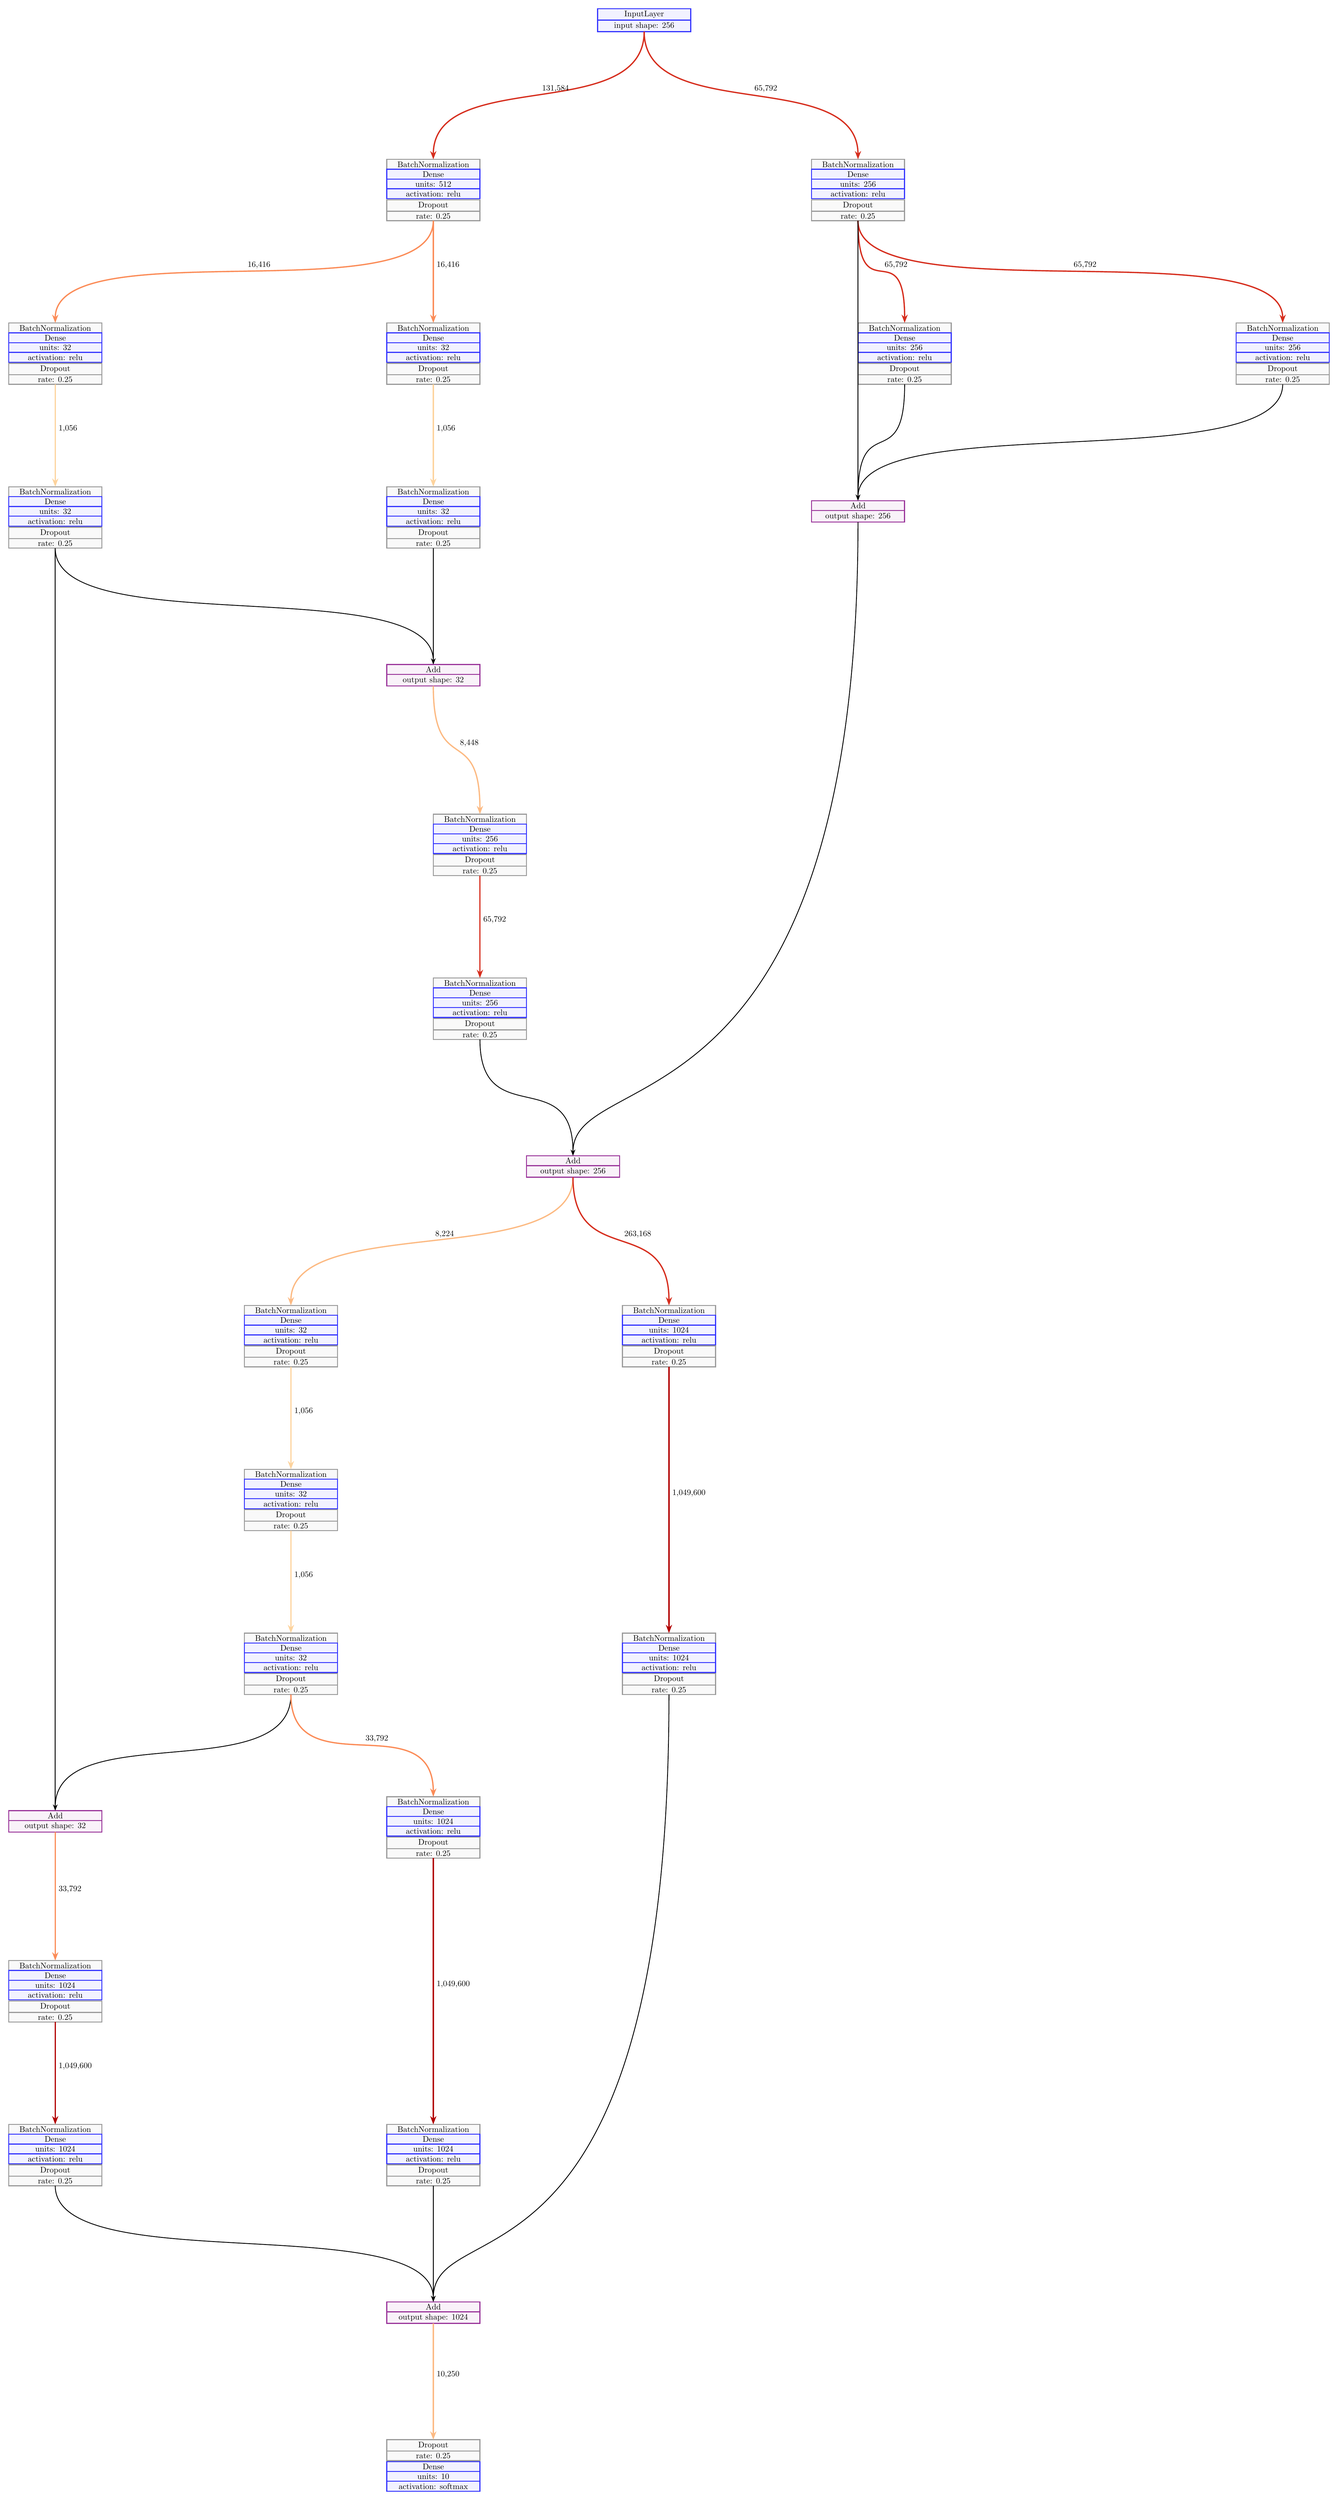
\begin{tikzpicture}[x=15.0pt, y=15.0pt, scale=2.0]
% style: major_grid
\tikzstyle{major_grid}=[black,step=20pt]
% style: minor_grid
\tikzstyle{minor_grid}=[very thin,step=10pt]
% style: defaultEdge
\tikzstyle{defaultEdge}=[thick,out=-90,in=90,out distance=1.5cm,in distance=1.5cm,looseness=1.5]
% style: defaultLabel
\tikzstyle{defaultLabel}=[auto,anchor=south west]
% style: operation_layer_style
\tikzstyle{operation_layer_style}=[rectangle split,rectangle split ignore empty parts,very thick,rectangle split parts=5,draw=violet!80,fill=violet!5,minimum width=4cm,outer sep=0cm,inner sep=2pt]
% style: pool_layer_style
\tikzstyle{pool_layer_style}=[rectangle split,rectangle split ignore empty parts,very thick,rectangle split parts=5,draw=brown!80,fill=brown!5,minimum width=4cm,outer sep=0cm,inner sep=2pt]
% style: utility_layer_style
\tikzstyle{utility_layer_style}=[rectangle split,rectangle split ignore empty parts,very thick,rectangle split parts=5,draw=gray!80,fill=gray!5,minimum width=4cm,outer sep=0cm,inner sep=2pt]
% style: default_layer_style
\tikzstyle{default_layer_style}=[rectangle split,rectangle split ignore empty parts,very thick,rectangle split parts=5,draw=blue!80,fill=blue!5,minimum width=4cm,outer sep=0cm,inner sep=2pt]
% style: misc_layer_style
\tikzstyle{misc_layer_style}=[rectangle split,rectangle split ignore empty parts,very thick,rectangle split parts=5,draw=teal!80,fill=teal!5,minimum width=4cm,outer sep=0cm,inner sep=2pt]

\definecolor{COLOR0}{RGB}{253,231,199}
\definecolor{COLOR1}{RGB}{253,211,157}
\definecolor{COLOR2}{RGB}{252,186,131}
\definecolor{COLOR3}{RGB}{251,140,88}
\definecolor{COLOR4}{RGB}{238,99,71}
\definecolor{COLOR5}{RGB}{214,46,30}
\definecolor{COLOR6}{RGB}{177,0,0}
% node group: input_1_group
% node: input_1
\node[default_layer_style] (input_1) at (23.99, 100.0)
    {
    \nodepart{one}{InputLayer}
    \nodepart{two}{input shape: 256}};
% end of node group: input_1_group

% node group: b_1_group
% node: batch_normalization_3
\node[utility_layer_style] (batch_normalization_3) at (15.4, 94.13)
    {
    \nodepart{one}{BatchNormalization}};
% node: dropout_3
\node[utility_layer_style] (dropout_3) at (15.4, 92.26)
    {
    \nodepart{one}{Dropout}
    \nodepart{two}{rate: 0.25}};
% node: b_1
\node[default_layer_style] (b_1) at (15.4, 93.33)
    {
    \nodepart{one}{Dense}
    \nodepart{two}{units: 512}
    \nodepart{three}{activation: relu}};
% end of node group: b_1_group

% node group: a_1_group
% node: batch_normalization
\node[utility_layer_style] (batch_normalization) at (32.7, 94.13)
    {
    \nodepart{one}{BatchNormalization}};
% node: dropout
\node[utility_layer_style] (dropout) at (32.7, 92.26)
    {
    \nodepart{one}{Dropout}
    \nodepart{two}{rate: 0.25}};
% node: a_1
\node[default_layer_style] (a_1) at (32.7, 93.33)
    {
    \nodepart{one}{Dense}
    \nodepart{two}{units: 256}
    \nodepart{three}{activation: relu}};
% end of node group: a_1_group

% node group: sum_a_group
% node: sum_a
\node[operation_layer_style] (sum_a) at (32.7, 80.0)
    {
    \nodepart{one}{Add}
    \nodepart{two}{output shape: 256}};
% end of node group: sum_a_group

% node group: b1_1_group
% node: batch_normalization_4
\node[utility_layer_style] (batch_normalization_4) at (15.4, 87.47)
    {
    \nodepart{one}{BatchNormalization}};
% node: dropout_4
\node[utility_layer_style] (dropout_4) at (15.4, 85.6)
    {
    \nodepart{one}{Dropout}
    \nodepart{two}{rate: 0.25}};
% node: b1_1
\node[default_layer_style] (b1_1) at (15.4, 86.67)
    {
    \nodepart{one}{Dense}
    \nodepart{two}{units: 32}
    \nodepart{three}{activation: relu}};
% end of node group: b1_1_group

% node group: b2_1_group
% node: batch_normalization_6
\node[utility_layer_style] (batch_normalization_6) at (0.0, 87.47)
    {
    \nodepart{one}{BatchNormalization}};
% node: dropout_6
\node[utility_layer_style] (dropout_6) at (0.0, 85.6)
    {
    \nodepart{one}{Dropout}
    \nodepart{two}{rate: 0.25}};
% node: b2_1
\node[default_layer_style] (b2_1) at (0.0, 86.67)
    {
    \nodepart{one}{Dense}
    \nodepart{two}{units: 32}
    \nodepart{three}{activation: relu}};
% end of node group: b2_1_group

% node group: a1_1_group
% node: batch_normalization_1
\node[utility_layer_style] (batch_normalization_1) at (34.6, 87.47)
    {
    \nodepart{one}{BatchNormalization}};
% node: dropout_1
\node[utility_layer_style] (dropout_1) at (34.6, 85.6)
    {
    \nodepart{one}{Dropout}
    \nodepart{two}{rate: 0.25}};
% node: a1_1
\node[default_layer_style] (a1_1) at (34.6, 86.67)
    {
    \nodepart{one}{Dense}
    \nodepart{two}{units: 256}
    \nodepart{three}{activation: relu}};
% end of node group: a1_1_group

% node group: a2_1_group
% node: batch_normalization_2
\node[utility_layer_style] (batch_normalization_2) at (50.0, 87.47)
    {
    \nodepart{one}{BatchNormalization}};
% node: dropout_2
\node[utility_layer_style] (dropout_2) at (50.0, 85.6)
    {
    \nodepart{one}{Dropout}
    \nodepart{two}{rate: 0.25}};
% node: a2_1
\node[default_layer_style] (a2_1) at (50.0, 86.67)
    {
    \nodepart{one}{Dense}
    \nodepart{two}{units: 256}
    \nodepart{three}{activation: relu}};
% end of node group: a2_1_group

% node group: sum_ab_group
% node: sum_ab
\node[operation_layer_style] (sum_ab) at (21.09, 53.33)
    {
    \nodepart{one}{Add}
    \nodepart{two}{output shape: 256}};
% end of node group: sum_ab_group

% node group: e_1_group
% node: batch_normalization_12
\node[utility_layer_style] (batch_normalization_12) at (9.6, 47.47)
    {
    \nodepart{one}{BatchNormalization}};
% node: dropout_12
\node[utility_layer_style] (dropout_12) at (9.6, 45.6)
    {
    \nodepart{one}{Dropout}
    \nodepart{two}{rate: 0.25}};
% node: e_1
\node[default_layer_style] (e_1) at (9.6, 46.67)
    {
    \nodepart{one}{Dense}
    \nodepart{two}{units: 32}
    \nodepart{three}{activation: relu}};
% end of node group: e_1_group

% node group: d_1_group
% node: batch_normalization_10
\node[utility_layer_style] (batch_normalization_10) at (25.0, 47.47)
    {
    \nodepart{one}{BatchNormalization}};
% node: dropout_10
\node[utility_layer_style] (dropout_10) at (25.0, 45.6)
    {
    \nodepart{one}{Dropout}
    \nodepart{two}{rate: 0.25}};
% node: d_1
\node[default_layer_style] (d_1) at (25.0, 46.67)
    {
    \nodepart{one}{Dense}
    \nodepart{two}{units: 1024}
    \nodepart{three}{activation: relu}};
% end of node group: d_1_group

% node group: b1_2_group
% node: batch_normalization_5
\node[utility_layer_style] (batch_normalization_5) at (15.4, 80.8)
    {
    \nodepart{one}{BatchNormalization}};
% node: dropout_5
\node[utility_layer_style] (dropout_5) at (15.4, 78.93)
    {
    \nodepart{one}{Dropout}
    \nodepart{two}{rate: 0.25}};
% node: b1_2
\node[default_layer_style] (b1_2) at (15.4, 80.0)
    {
    \nodepart{one}{Dense}
    \nodepart{two}{units: 32}
    \nodepart{three}{activation: relu}};
% end of node group: b1_2_group

% node group: b2_2_group
% node: batch_normalization_7
\node[utility_layer_style] (batch_normalization_7) at (0.0, 80.8)
    {
    \nodepart{one}{BatchNormalization}};
% node: dropout_7
\node[utility_layer_style] (dropout_7) at (0.0, 78.93)
    {
    \nodepart{one}{Dropout}
    \nodepart{two}{rate: 0.25}};
% node: b2_2
\node[default_layer_style] (b2_2) at (0.0, 80.0)
    {
    \nodepart{one}{Dense}
    \nodepart{two}{units: 32}
    \nodepart{three}{activation: relu}};
% end of node group: b2_2_group

% node group: sum_b_group
% node: sum_b
\node[operation_layer_style] (sum_b) at (15.4, 73.33)
    {
    \nodepart{one}{Add}
    \nodepart{two}{output shape: 32}};
% end of node group: sum_b_group

% node group: sum_b2_e_group
% node: sum_b2_e
\node[operation_layer_style] (sum_b2_e) at (0.0, 26.67)
    {
    \nodepart{one}{Add}
    \nodepart{two}{output shape: 32}};
% end of node group: sum_b2_e_group

% node group: e_2_group
% node: batch_normalization_13
\node[utility_layer_style] (batch_normalization_13) at (9.6, 40.8)
    {
    \nodepart{one}{BatchNormalization}};
% node: dropout_13
\node[utility_layer_style] (dropout_13) at (9.6, 38.93)
    {
    \nodepart{one}{Dropout}
    \nodepart{two}{rate: 0.25}};
% node: e_2
\node[default_layer_style] (e_2) at (9.6, 40.0)
    {
    \nodepart{one}{Dense}
    \nodepart{two}{units: 32}
    \nodepart{three}{activation: relu}};
% end of node group: e_2_group

% node group: d_2_group
% node: batch_normalization_11
\node[utility_layer_style] (batch_normalization_11) at (25.0, 34.13)
    {
    \nodepart{one}{BatchNormalization}};
% node: dropout_11
\node[utility_layer_style] (dropout_11) at (25.0, 32.26)
    {
    \nodepart{one}{Dropout}
    \nodepart{two}{rate: 0.25}};
% node: d_2
\node[default_layer_style] (d_2) at (25.0, 33.33)
    {
    \nodepart{one}{Dense}
    \nodepart{two}{units: 1024}
    \nodepart{three}{activation: relu}};
% end of node group: d_2_group

% node group: b_2_group
% node: batch_normalization_8
\node[utility_layer_style] (batch_normalization_8) at (17.3, 67.47)
    {
    \nodepart{one}{BatchNormalization}};
% node: dropout_8
\node[utility_layer_style] (dropout_8) at (17.3, 65.6)
    {
    \nodepart{one}{Dropout}
    \nodepart{two}{rate: 0.25}};
% node: b_2
\node[default_layer_style] (b_2) at (17.3, 66.67)
    {
    \nodepart{one}{Dense}
    \nodepart{two}{units: 256}
    \nodepart{three}{activation: relu}};
% end of node group: b_2_group

% node group: e2_1_group
% node: batch_normalization_17
\node[utility_layer_style] (batch_normalization_17) at (0.0, 20.8)
    {
    \nodepart{one}{BatchNormalization}};
% node: dropout_17
\node[utility_layer_style] (dropout_17) at (0.0, 18.93)
    {
    \nodepart{one}{Dropout}
    \nodepart{two}{rate: 0.25}};
% node: e2_1
\node[default_layer_style] (e2_1) at (0.0, 20.0)
    {
    \nodepart{one}{Dense}
    \nodepart{two}{units: 1024}
    \nodepart{three}{activation: relu}};
% end of node group: e2_1_group

% node group: sum_d_e_group
% node: sum_d_e
\node[operation_layer_style] (sum_d_e) at (15.4, 6.67)
    {
    \nodepart{one}{Add}
    \nodepart{two}{output shape: 1024}};
% end of node group: sum_d_e_group

% node group: e_3_group
% node: batch_normalization_14
\node[utility_layer_style] (batch_normalization_14) at (9.6, 34.13)
    {
    \nodepart{one}{BatchNormalization}};
% node: dropout_14
\node[utility_layer_style] (dropout_14) at (9.6, 32.26)
    {
    \nodepart{one}{Dropout}
    \nodepart{two}{rate: 0.25}};
% node: e_3
\node[default_layer_style] (e_3) at (9.6, 33.33)
    {
    \nodepart{one}{Dense}
    \nodepart{two}{units: 32}
    \nodepart{three}{activation: relu}};
% end of node group: e_3_group

% node group: output_group
% node: dropout_out
\node[utility_layer_style] (dropout_out) at (15.4, 1.07)
    {
    \nodepart{one}{Dropout}
    \nodepart{two}{rate: 0.25}};
% node: output
\node[default_layer_style] (output) at (15.4, 0.0)
    {
    \nodepart{one}{Dense}
    \nodepart{two}{units: 10}
    \nodepart{three}{activation: softmax}};
% end of node group: output_group

% node group: b_3_group
% node: batch_normalization_9
\node[utility_layer_style] (batch_normalization_9) at (17.3, 60.8)
    {
    \nodepart{one}{BatchNormalization}};
% node: dropout_9
\node[utility_layer_style] (dropout_9) at (17.3, 58.93)
    {
    \nodepart{one}{Dropout}
    \nodepart{two}{rate: 0.25}};
% node: b_3
\node[default_layer_style] (b_3) at (17.3, 60.0)
    {
    \nodepart{one}{Dense}
    \nodepart{two}{units: 256}
    \nodepart{three}{activation: relu}};
% end of node group: b_3_group

% node group: e2_2_group
% node: batch_normalization_18
\node[utility_layer_style] (batch_normalization_18) at (0.0, 14.13)
    {
    \nodepart{one}{BatchNormalization}};
% node: dropout_18
\node[utility_layer_style] (dropout_18) at (0.0, 12.26)
    {
    \nodepart{one}{Dropout}
    \nodepart{two}{rate: 0.25}};
% node: e2_2
\node[default_layer_style] (e2_2) at (0.0, 13.33)
    {
    \nodepart{one}{Dense}
    \nodepart{two}{units: 1024}
    \nodepart{three}{activation: relu}};
% end of node group: e2_2_group

% node group: e1_1_group
% node: batch_normalization_15
\node[utility_layer_style] (batch_normalization_15) at (15.4, 27.47)
    {
    \nodepart{one}{BatchNormalization}};
% node: dropout_15
\node[utility_layer_style] (dropout_15) at (15.4, 25.6)
    {
    \nodepart{one}{Dropout}
    \nodepart{two}{rate: 0.25}};
% node: e1_1
\node[default_layer_style] (e1_1) at (15.4, 26.67)
    {
    \nodepart{one}{Dense}
    \nodepart{two}{units: 1024}
    \nodepart{three}{activation: relu}};
% end of node group: e1_1_group

% node group: e1_2_group
% node: batch_normalization_16
\node[utility_layer_style] (batch_normalization_16) at (15.4, 14.13)
    {
    \nodepart{one}{BatchNormalization}};
% node: dropout_16
\node[utility_layer_style] (dropout_16) at (15.4, 12.26)
    {
    \nodepart{one}{Dropout}
    \nodepart{two}{rate: 0.25}};
% node: e1_2
\node[default_layer_style] (e1_2) at (15.4, 13.33)
    {
    \nodepart{one}{Dense}
    \nodepart{two}{units: 1024}
    \nodepart{three}{activation: relu}};
% end of node group: e1_2_group

% edge from input_1 to batch_normalization_3
\draw[-Stealth, defaultEdge, in distance=2.0cm,out distance=2.0cm,draw=COLOR5,line width=1.6pt] (input_1) to node [defaultLabel] {131,584} (batch_normalization_3);

% edge from input_1 to batch_normalization
\draw[-Stealth, defaultEdge, in distance=2.0cm,out distance=2.0cm,draw=COLOR5,line width=1.6pt] (input_1) to node [defaultLabel] {65,792} (batch_normalization);

% edge from dropout_3 to batch_normalization_4
\draw[-Stealth, defaultEdge, in distance=2.0cm,out distance=2.0cm,draw=COLOR3,line width=1.6pt] (dropout_3) to node [defaultLabel] {16,416} (batch_normalization_4);

% edge from dropout_3 to batch_normalization_6
\draw[-Stealth, defaultEdge, in distance=2.0cm,out distance=2.0cm,draw=COLOR3,line width=1.6pt] (dropout_3) to node [defaultLabel] {16,416} (batch_normalization_6);

% edge from dropout to batch_normalization_1
\draw[-Stealth, defaultEdge, in distance=2.0cm,out distance=2.0cm,draw=COLOR5,line width=1.6pt] (dropout) to node [defaultLabel] {65,792} (batch_normalization_1);

% edge from dropout to batch_normalization_2
\draw[-Stealth, defaultEdge, in distance=2.0cm,out distance=2.0cm,draw=COLOR5,line width=1.6pt] (dropout) to node [defaultLabel] {65,792} (batch_normalization_2);

% edge from dropout to sum_a
\draw[-Stealth, defaultEdge, in distance=2.0cm,out distance=2.0cm,draw=black,line width=1pt] (dropout) to node [defaultLabel] {} (sum_a);

% edge from sum_a to sum_ab
\draw[-Stealth, defaultEdge, in distance=2.0cm,out distance=13.34cm,draw=black,line width=1pt] (sum_a) to node [defaultLabel] {} (sum_ab);

% edge from dropout_4 to batch_normalization_5
\draw[-Stealth, defaultEdge, in distance=2.0cm,out distance=2.0cm,draw=COLOR1,line width=1.6pt] (dropout_4) to node [defaultLabel] {1,056} (batch_normalization_5);

% edge from dropout_6 to batch_normalization_7
\draw[-Stealth, defaultEdge, in distance=2.0cm,out distance=2.0cm,draw=COLOR1,line width=1.6pt] (dropout_6) to node [defaultLabel] {1,056} (batch_normalization_7);

% edge from dropout_1 to sum_a
\draw[-Stealth, defaultEdge, in distance=2.0cm,out distance=2.0cm,draw=black,line width=1pt] (dropout_1) to node [defaultLabel] {} (sum_a);

% edge from dropout_2 to sum_a
\draw[-Stealth, defaultEdge, in distance=2.0cm,out distance=2.0cm,draw=black,line width=1pt] (dropout_2) to node [defaultLabel] {} (sum_a);

% edge from sum_ab to batch_normalization_12
\draw[-Stealth, defaultEdge, in distance=2.0cm,out distance=2.0cm,draw=COLOR2,line width=1.6pt] (sum_ab) to node [defaultLabel] {8,224} (batch_normalization_12);

% edge from sum_ab to batch_normalization_10
\draw[-Stealth, defaultEdge, in distance=2.0cm,out distance=2.0cm,draw=COLOR5,line width=1.6pt] (sum_ab) to node [defaultLabel] {263,168} (batch_normalization_10);

% edge from dropout_12 to batch_normalization_13
\draw[-Stealth, defaultEdge, in distance=2.0cm,out distance=2.0cm,draw=COLOR1,line width=1.6pt] (dropout_12) to node [defaultLabel] {1,056} (batch_normalization_13);

% edge from dropout_10 to batch_normalization_11
\draw[-Stealth, defaultEdge, in distance=4.0cm,out distance=4.0cm,draw=COLOR6,line width=1.6pt] (dropout_10) to node [defaultLabel] {1,049,600} (batch_normalization_11);

% edge from dropout_5 to sum_b
\draw[-Stealth, defaultEdge, in distance=2.0cm,out distance=2.0cm,draw=black,line width=1pt] (dropout_5) to node [defaultLabel] {} (sum_b);

% edge from dropout_7 to sum_b
\draw[-Stealth, defaultEdge, in distance=2.0cm,out distance=2.0cm,draw=black,line width=1pt] (dropout_7) to node [defaultLabel] {} (sum_b);

% edge from dropout_7 to sum_b2_e
\draw[-Stealth, defaultEdge, in distance=2.0cm,out distance=2.0cm,draw=black,line width=1pt] (dropout_7) to node [defaultLabel] {} (sum_b2_e);

% edge from sum_b to batch_normalization_8
\draw[-Stealth, defaultEdge, in distance=2.0cm,out distance=2.0cm,draw=COLOR2,line width=1.6pt] (sum_b) to node [defaultLabel] {8,448} (batch_normalization_8);

% edge from sum_b2_e to batch_normalization_17
\draw[-Stealth, defaultEdge, in distance=2.0cm,out distance=2.0cm,draw=COLOR3,line width=1.6pt] (sum_b2_e) to node [defaultLabel] {33,792} (batch_normalization_17);

% edge from dropout_13 to batch_normalization_14
\draw[-Stealth, defaultEdge, in distance=2.0cm,out distance=2.0cm,draw=COLOR1,line width=1.6pt] (dropout_13) to node [defaultLabel] {1,056} (batch_normalization_14);

% edge from dropout_11 to sum_d_e
\draw[-Stealth, defaultEdge, in distance=2.0cm,out distance=13.33cm,draw=black,line width=1pt] (dropout_11) to node [defaultLabel] {} (sum_d_e);

% edge from dropout_8 to batch_normalization_9
\draw[-Stealth, defaultEdge, in distance=2.0cm,out distance=2.0cm,draw=COLOR5,line width=1.6pt] (dropout_8) to node [defaultLabel] {65,792} (batch_normalization_9);

% edge from dropout_17 to batch_normalization_18
\draw[-Stealth, defaultEdge, in distance=2.0cm,out distance=2.0cm,draw=COLOR6,line width=1.6pt] (dropout_17) to node [defaultLabel] {1,049,600} (batch_normalization_18);

% edge from sum_d_e to dropout_out
\draw[-Stealth, defaultEdge, in distance=2.0cm,out distance=2.0cm,draw=COLOR2,line width=1.6pt] (sum_d_e) to node [defaultLabel] {10,250} (dropout_out);

% edge from dropout_14 to sum_b2_e
\draw[-Stealth, defaultEdge, in distance=2.0cm,out distance=2.0cm,draw=black,line width=1pt] (dropout_14) to node [defaultLabel] {} (sum_b2_e);

% edge from dropout_14 to batch_normalization_15
\draw[-Stealth, defaultEdge, in distance=2.0cm,out distance=2.0cm,draw=COLOR3,line width=1.6pt] (dropout_14) to node [defaultLabel] {33,792} (batch_normalization_15);

% edge from dropout_9 to sum_ab
\draw[-Stealth, defaultEdge, in distance=2.0cm,out distance=2.0cm,draw=black,line width=1pt] (dropout_9) to node [defaultLabel] {} (sum_ab);

% edge from dropout_18 to sum_d_e
\draw[-Stealth, defaultEdge, in distance=2.0cm,out distance=2.0cm,draw=black,line width=1pt] (dropout_18) to node [defaultLabel] {} (sum_d_e);

% edge from dropout_15 to batch_normalization_16
\draw[-Stealth, defaultEdge, in distance=4.0cm,out distance=4.0cm,draw=COLOR6,line width=1.6pt] (dropout_15) to node [defaultLabel] {1,049,600} (batch_normalization_16);

% edge from dropout_16 to sum_d_e
\draw[-Stealth, defaultEdge, in distance=2.0cm,out distance=2.0cm,draw=black,line width=1pt] (dropout_16) to node [defaultLabel] {} (sum_d_e);

\end{tikzpicture}\end{document}